\documentclass[12pt,fleqn]{article}
\setlength{\parindent}{0pt}
\usepackage{graphicx}
\usepackage{cancel}
\usepackage{listings}
\usepackage[latin5]{inputenc}
\usepackage{color}
\setlength{\parskip}{8pt}
\setlength{\parsep}{0pt}
\setlength{\headsep}{0pt}
\setlength{\topskip}{0pt}
\setlength{\topmargin}{0pt}
\setlength{\topsep}{0pt}
\setlength{\partopsep}{0pt}
\setlength{\mathindent}{0cm}

\begin{document}
Ders 2

Karakteristik Egriler Metodu

Bu metot katsayilari sabit olmayan 1. derece, lineer PDE cozmemize yardim
eder. PDE su formdadir

\[ \frac{\partial u}{\partial x} + 
p(x,y) \frac{\partial u}{\partial y} = 0 
\ \ \ (*)
 \]

ve $p(x,y)$, $x,y$ degiskenlerinin bir fonksiyonudur. 

Ustteki denklemi iki vektorun noktasal carpimi olarak ta gorebiliriz. 

\[ 
<\frac{\partial u}{\partial x}, \frac{\partial u}{\partial y}> \cdot 
<1,p(x,y)> = 0
 \]

Bu acidan bakinca yukaridaki ifade yeni bir sey soyluyor, $u$'nun
$<1,p(x,y)>$ vektorune gore yonsel turevinin sifir oldugunu soyluyor, yani
o yonde hicbir degisim yok. 

Simdi tek basina $<1,p(x,y)>$ vektorunu dusunelim, her degisik $x,y$ icin
bu vektorler bir vektor alani olusturur, bu alandaki vektorleri bir egrinin
``belli bir noktadaki egimini gosterdigi'' seklinde alabiliriz. O
noktalardaki egim $p(x,y) / 1$ olacaktir dogal olarak, o zaman bu egriler
icin soyle bir basit diferansiyel denklem (ODE) yazabiliriz.

\[ \frac{dy}{dx} = \frac{p(x,y)}{1} \]

ya da

\[ \frac{dy}{dx} = p(x,y) 
\ \ \ (**)
\]

Bu ODE bir yon alani (direction field) olusturur (bkz MIT OCW ODE Ders 1).

Simdi geri adim atip her seye tekrar bakalim. (*) diyor ki $x,y$ noktasinda
$u$'nun $<1,p(x,y)>$ yonundeki yonsel turevi sifir. Yani $x,y$ noktasinda
$<1,p(x,y)>$ yonunde ilerlersek $u$ hic degismeyecek. 

Ayni zamanda $<1,p(x,y)>$ vektorleri (**) icin bir yonsel alan da
tanimliyor!  Bilindigi gibi (**) denklemi cozum egrileri (solution curves)
ortaya cikartir, ve ne raslanti ki (!) bu cozum egrilerinin her birinde
(*)'deki $u$ sabit kalir. 

Ornek 

\[ \frac{\partial u}{\partial x} + 
x \frac{\partial u}{\partial y} = 0 
 \]

Yani $p(x,y) = x$. O zaman 

\[ \frac{dy}{dx} = x \]

denklemini cozeriz, ve 

\[ y = \frac{1}{2}x^2 + C \]

karakteristik egrilerini elde ederiz. Tekrar duzenlersek

\[ y - \frac{1}{2}x^2 = C \]

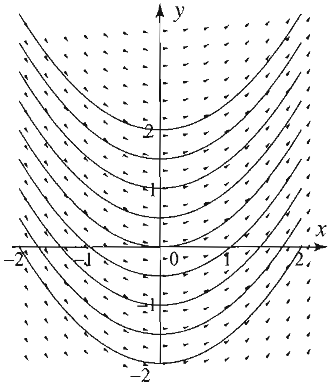
\includegraphics[height=4cm]{2_1.png}

O zaman PDE'nin genel cozumu 

\[ u(x,y) = f(C) = f(y - \frac{1}{2}x^2) \]

diyebiliriz, $f$ rasgele bir fonksiyondur, soylenmeye ugrasilan farkli
sabitlere tekabul eden $u$'lardir. PDE cozumu $u$'nun sabite esit olmasiyla
alakali cunku PDE'yi yonsel turev olarak temsil edince bu sonuca
variyoruz. Ustteki denklem de karakteristik egriler acisindan gelerek o
sabiti bize sagliyor.

$f$'in genel cozum oldugunu ana denklemde yerine koyarak test edebiliriz.

Ornek 

\[ u_x + yu_y = 0 \]

O zaman 

\[ \frac{dy}{dx} = y \]

\[ y = Ce^x \]

ya da

\[  C = e^{-x}y\]

Genel cozum 

\[ u(x,y) = f(C) = f(e^{-x}y) \]

PDE icinde yerine koyarak sonucu kontrol edelim

\[ u_x + yu_y = 
-f'(e^{-x}y)e^{-x}y + y f'(e^{-x}y) e^{-x} = 0
 \]

Isi Denklemi 

\[ u_{tt} = c^2 u_{xx} \]

isi denklemi olarak bilinir. Bir diger sekilde 

\[ u_{tt} - c^2 u_{xx} = 0\]

Bu denklemi operatorlerin faktorize edilmis hali olarak gormek mumkundur. 

\[ u_{tt} - c^2 u_{xx} = 
\bigg( \frac{\partial }{\partial t} - c \frac{\partial }{\partial x} \bigg)
\bigg( \frac{\partial }{\partial t} + c \frac{\partial }{\partial x} \bigg)
u = 0
\ \ \ (***)
\]

Esitligin sag tarafindaki operatorler hakikaten isi denklemine tekabul
ediyor mu? Kontrol edelim, 

\[ \bigg( \frac{\partial }{\partial t} + c \frac{\partial }{\partial x}
\bigg) u = 
\frac{\partial u}{\partial t} + c \frac{\partial u}{\partial x}
\]

Sag tarafa bir daha operator uygulayalim (bu sefer eksi olan operator),
yani sunu hesaplayalim

\[ 
\bigg( \frac{\partial }{\partial t} - c \frac{\partial }{\partial x} \bigg)
\frac{\partial u}{\partial t} + c \frac{\partial u}{\partial x} 
 \]

\[ = 
\frac{\partial ^2 u}{\partial t^2} + 
c \frac{\partial u}{\partial x \partial t} - 
c \frac{\partial u}{\partial t \partial x} - 
c^2\frac{\partial ^2 u}{\partial x^2} 
 \]

$u_{xt} = u_{tx}$ olduguna gore ortadaki iki terim iptal olur

\[ = 
\frac{\partial ^2 u}{\partial t^2} -
c^2\frac{\partial ^2 u}{\partial x^2} 
 \]

Acilimi ispatlamis olduk. 

Simdi isi denkleminin operator acilimini, faktorize edilmis halini
dusunursek, o zaman iddia ediyorum ki genel cozum su halde

\[ u(x,t) = f(x+ct) + g(x-ct) \]

ki $f$ ve $g$ tek degiskenli rasgele birer fonksiyon. 

Ispat

(***) sebebiyle ve eger $v$'nin $v = u_t + cu_x$ oldugunu farzedersek, o zaman 

\[ v_t - cv_x = 0 \]

dogru olmalidir. O zaman elimizde iki tane birinci derece denklem vardir

\[ v_t - cv_x = 0 \]

\[ u_t + cu_x = v \]

Simdi bu denklemleri teker teker cozelim. 1. Ders'ten biliyoruz ki iki
ustteki denklemin cozumu 

\[ v(x,t) = h(x+ ct) \]

ki $h$ herhangi bir fonksiyon. Simdi diger formulu cozmek lazim, ki onun
da formu

\[ u_t + cu_x = h(x + ct)  \]

Cozmek derken ustteki denkleme gore $u(x,t)$'yi bulmak gerekli. 

















\end{document}
